%  LaTeX support: latex@mdpi.com 
%  For support, please attach all files needed for compiling as well as the log file, and specify your operating system, LaTeX version, and LaTeX editor.

%=================================================================
\documentclass[sensors,article,submit,pdftex,moreauthors]{Definitions/mdpi} 
% For posting an early version of this manuscript as a preprint, you may use "preprints" as the journal and change "submit" to "accept". The document class line would be, e.g., \documentclass[preprints,article,accept,moreauthors,pdftex]{mdpi}. This is especially recommended for submission to arXiv, where line numbers should be removed before posting. For preprints.org, the editorial staff will make this change immediately prior to posting.

%--------------------
% Class Options:
%--------------------
%----------
% journal
%----------
% Choose between the following MDPI journals:
% acoustics, actuators, addictions, admsci, adolescents, aerospace, agriculture, agriengineering, agronomy, ai, algorithms, allergies, alloys, analytica, animals, antibiotics, antibodies, antioxidants, applbiosci, appliedchem, appliedmath, applmech, applmicrobiol, applnano, applsci, aquacj, architecture, arts, asc, asi, astronomy, atmosphere, atoms, audiolres, automation, axioms, bacteria, batteries, bdcc, behavsci, beverages, biochem, bioengineering, biologics, biology, biomass, biomechanics, biomed, biomedicines, biomedinformatics, biomimetics, biomolecules, biophysica, biosensors, biotech, birds, bloods, blsf, brainsci, breath, buildings, businesses, cancers, carbon, cardiogenetics, catalysts, cells, ceramics, challenges, chemengineering, chemistry, chemosensors, chemproc, children, chips, cimb, civileng, cleantechnol, climate, clinpract, clockssleep, cmd, coasts, coatings, colloids, colorants, commodities, compounds, computation, computers, condensedmatter, conservation, constrmater, cosmetics, covid, crops, cryptography, crystals, csmf, ctn, curroncol, currophthalmol, cyber, dairy, data, dentistry, dermato, dermatopathology, designs, diabetology, diagnostics, dietetics, digital, disabilities, diseases, diversity, dna, drones, dynamics, earth, ebj, ecologies, econometrics, economies, education, ejihpe, electricity, electrochem, electronicmat, electronics, encyclopedia, endocrines, energies, eng, engproc, ent, entomology, entropy, environments, environsciproc, epidemiologia, epigenomes, est, fermentation, fibers, fintech, fire, fishes, fluids, foods, forecasting, forensicsci, forests, foundations, fractalfract, fuels, futureinternet, futureparasites, futurepharmacol, futurephys, futuretransp, galaxies, games, gases, gastroent, gastrointestdisord, gels, genealogy, genes, geographies, geohazards, geomatics, geosciences, geotechnics, geriatrics, hazardousmatters, healthcare, hearts, hemato, heritage, highthroughput, histories, horticulturae, humanities, humans, hydrobiology, hydrogen, hydrology, hygiene, idr, ijerph, ijfs, ijgi, ijms, ijns, ijtm, ijtpp, immuno, informatics, information, infrastructures, inorganics, insects, instruments, inventions, iot, j, jal, jcdd, jcm, jcp, jcs, jdb, jeta, jfb, jfmk, jimaging, jintelligence, jlpea, jmmp, jmp, jmse, jne, jnt, jof, joitmc, jor, journalmedia, jox, jpm, jrfm, jsan, jtaer, jzbg, kidney, kidneydial, knowledge, land, languages, laws, life, liquids, literature, livers, logics, logistics, lubricants, lymphatics, machines, macromol, magnetism, magnetochemistry, make, marinedrugs, materials, materproc, mathematics, mca, measurements, medicina, medicines, medsci, membranes, merits, metabolites, metals, meteorology, methane, metrology, micro, microarrays, microbiolres, micromachines, microorganisms, microplastics, minerals, mining, modelling, molbank, molecules, mps, msf, mti, muscles, nanoenergyadv, nanomanufacturing, nanomaterials, ncrna, network, neuroglia, neurolint, neurosci, nitrogen, notspecified, nri, nursrep, nutraceuticals, nutrients, obesities, oceans, ohbm, onco, oncopathology, optics, oral, organics, organoids, osteology, oxygen, parasites, parasitologia, particles, pathogens, pathophysiology, pediatrrep, pharmaceuticals, pharmaceutics, pharmacoepidemiology, pharmacy, philosophies, photochem, photonics, phycology, physchem, physics, physiologia, plants, plasma, pollutants, polymers, polysaccharides, poultry, powders, preprints, proceedings, processes, prosthesis, proteomes, psf, psych, psychiatryint, psychoactives, publications, quantumrep, quaternary, qubs, radiation, reactions, recycling, regeneration, religions, remotesensing, reports, reprodmed, resources, rheumato, risks, robotics, ruminants, safety, sci, scipharm, seeds, sensors, separations, sexes, signals, sinusitis, skins, smartcities, sna, societies, socsci, software, soilsystems, solar, solids, sports, standards, stats, stresses, surfaces, surgeries, suschem, sustainability, symmetry, synbio, systems, taxonomy, technologies, telecom, test, textiles, thalassrep, thermo, tomography, tourismhosp, toxics, toxins, transplantology, transportation, traumacare, traumas, tropicalmed, universe, urbansci, uro, vaccines, vehicles, venereology, vetsci, vibration, viruses, vision, waste, water, wem, wevj, wind, women, world, youth, zoonoticdis 

%---------
% article
%---------
% The default type of manuscript is "article", but can be replaced by: 
% abstract, addendum, article, book, bookreview, briefreport, casereport, comment, commentary, communication, conferenceproceedings, correction, conferencereport, entry, expressionofconcern, extendedabstract, datadescriptor, editorial, essay, erratum, hypothesis, interestingimage, obituary, opinion, projectreport, reply, retraction, review, perspective, protocol, shortnote, studyprotocol, systematicreview, supfile, technicalnote, viewpoint, guidelines, registeredreport, tutorial
% supfile = supplementary materials

%----------
% submit
%----------
% The class option "submit" will be changed to "accept" by the Editorial Office when the paper is accepted. This will only make changes to the frontpage (e.g., the logo of the journal will get visible), the headings, and the copyright information. Also, line numbering will be removed. Journal info and pagination for accepted papers will also be assigned by the Editorial Office.

%------------------
% moreauthors
%------------------
% If there is only one author the class option oneauthor should be used. Otherwise use the class option moreauthors.

%---------
% pdftex
%---------
% The option pdftex is for use with pdfLaTeX. If eps figures are used, remove the option pdftex and use LaTeX and dvi2pdf.

%=================================================================
% MDPI internal commands
\firstpage{1} 
\makeatletter 
\setcounter{page}{\@firstpage} 
\makeatother
\pubvolume{1}
\issuenum{1}
\articlenumber{0}
\pubyear{2022}
\copyrightyear{2022}
%\externaleditor{Academic Editor: Firstname Lastname}
\datereceived{} 
%\daterevised{} % Only for the journal Acoustics
\dateaccepted{} 
\datepublished{} 
%\datecorrected{} % Corrected papers include a "Corrected: XXX" date in the original paper.
%\dateretracted{} % Corrected papers include a "Retracted: XXX" date in the original paper.
\hreflink{https://doi.org/} % If needed use \linebreak
%\doinum{}
%------------------------------------------------------------------
% The following line should be uncommented if the LaTeX file is uploaded to arXiv.org
%\pdfoutput=1

%=================================================================
% Add packages and commands here. The following packages are loaded in our class file: fontenc, inputenc, calc, indentfirst, fancyhdr, graphicx, epstopdf, lastpage, ifthen, lineno, float, amsmath, setspace, enumitem, mathpazo, booktabs, titlesec, etoolbox, tabto, xcolor, soul, multirow, microtype, tikz, totcount, changepage, attrib, upgreek, cleveref, amsthm, hyphenat, natbib, hyperref, footmisc, url, geometry, newfloat, caption
\usepackage{makecell}
\usepackage{placeins}
\usepackage{amsmath}
\usepackage{comment}

%=================================================================
%% Please use the following mathematics environments: Theorem, Lemma, Corollary, Proposition, Characterization, Property, Problem, Example, ExamplesandDefinitions, Hypothesis, Remark, Definition, Notation, Assumption
%% For proofs, please use the proof environment (the amsthm package is loaded by the MDPI class).

%=================================================================
% Full title of the paper (Capitalized)
\Title{DIAGNOSTIC SUPPORT OF SKIN LESION
	CLASSIFICATION USING CNN AND SOFT
	ATTENTION}

% MDPI internal command: Title for citation in the left column
\TitleCitation{DIAGNOSTIC SUPPORT OF SKIN LESION
	CLASSIFICATION USING CNN AND SOFT
	ATTENTION}

% Author Orchid ID: enter ID or remove command
\newcommand{\orcidauthorA}{0000-0002-2566-5637} % Add \orcidA{} behind the author's name
%\newcommand{\orcidauthorB}{0000-0000-0000-000X} % Add \orcidB{} behind the author's name

% Authors, for the paper (add full first names)
\Author{Khoi Do Hoang$^{
		1,\dagger,%\ddagger
	}$\orcidA{}*}

%\longauthorlist{yes}

% MDPI internal command: Authors, for metadata in PDF
\AuthorNames{Khoi Do}

% MDPI internal command: Authors, for citation in the left column
\AuthorCitation{Do, K.}
% If this is a Chicago style journal: Lastname, Firstname, Firstname Lastname, and Firstname Lastname.

% Affiliations / Addresses (Add [1] after \address if there is only one affiliation.)

\address{
$^{1}$ \quad Viet Dung Nguyen; dung.nguyenviet1@hust.edu.vn\\
$^{2}$ \quad Khoi Do Hoang; khoi.dh200332@sis.hust.edu.vn}

% Contact information of the corresponding author
\corres{Correspondence: khoido8899@gmail.com; Tel.: +84-9360-192-58}

% Current address and/or shared authorship
\firstnote{Current address: 1st Dai Co Viet Street, Ha Noi, Viet Nam} 
\secondnote{}
% The commands \thirdnote{} till \eighthnote{} are available for further notes 

%\simplesumm{} % Simple summary

%\conference{} % An extended version of a conference paper

% Abstract (Do not insert blank lines, i.e. \\) 
\abstract{Today, the rapid development of industrial zones leads to an increased incidence of skin	diseases because of polluted air. According to a report by the American Cancer Society, it is estimated that in 2022 there will be about 100,000 people suffering from skin cancer and more than 7600 of these people will not survive. In the context that doctors at provincial hospitals and health facilities are overloaded, doctors at lower levels lack experience and having	a tool to support doctors in the process of diagnosing skin diseases quickly and accurately is essential. Along with the strong development of artificial intelligence technologies, many solutions and tools to support the diagnosis of skin diseases have been researched and developed. These include DenseNet, InceptionNet, ResNet, NasNet, SeNet, EfficientNet, VGGNet. In this study, another approach to building tools to aid in the diagnosis of skin pathologies is proposed. SOTA (state of the art) models DenseNet, InceptionNet, ResNet, NasNet, MobileNet combined with Soft-Attention are used as backbone. In addition, personal information such as age and gender are also used. In addition, a new loss function	that takes into account the imbalance of the data is also proposed. Experimental results on dataset HAM10000 show that using InceptionResNetV2 with Soft-Attention and new loss function gives 90 percent accuracy, mean of precision, f1-score, recall-score, and AUC scores of 0.81, 0.81, 0.82, and 0.989, respectively, are improvements compared to published indexes. Besides, using MobileNetV3Large combined with Soft-Attention and new loss function, even though the number of parameters is 11 times less, the number of floors is 4 times less, it achieves 86 percent accuracy and 30 times faster diagnosis.}

% Keywords
\keyword{AI Diagnosis, Skin Sancer, Skin Lesion
	Classification, Deep Learning, Machine Learning)} 

% The fields PACS, MSC, and JEL may be left empty or commented out if not applicable
%\PACS{J0101}
%\MSC{}
%\JEL{}

%%%%%%%%%%%%%%%%%%%%%%%%%%%%%%%%%%%%%%%%%%
% Only for the journal Diversity
%\LSID{\url{http://}}

%%%%%%%%%%%%%%%%%%%%%%%%%%%%%%%%%%%%%%%%%%
% Only for the journal Applied Sciences
%\featuredapplication{Authors are encouraged to provide a concise description of the specific application or a potential application of the work. This section is not mandatory.}
%%%%%%%%%%%%%%%%%%%%%%%%%%%%%%%%%%%%%%%%%%

%%%%%%%%%%%%%%%%%%%%%%%%%%%%%%%%%%%%%%%%%%
% Only for the journal Data
%\dataset{DOI number or link to the deposited data set if the data set is published separately. If the data set shall be published as a supplement to this paper, this field will be filled by the journal editors. In this case, please submit the data set as a supplement.}
%\datasetlicense{License under which the data set is made available (CC0, CC-BY, CC-BY-SA, CC-BY-NC, etc.)}

%%%%%%%%%%%%%%%%%%%%%%%%%%%%%%%%%%%%%%%%%%
% Only for the journal Toxins
%\keycontribution{The breakthroughs or highlights of the manuscript. Authors can write one or two sentences to describe the most important part of the paper.}

%%%%%%%%%%%%%%%%%%%%%%%%%%%%%%%%%%%%%%%%%%
% Only for the journal Encyclopedia
%\encyclopediadef{For entry manuscripts only: please provide a brief overview of the entry title instead of an abstract.}

%%%%%%%%%%%%%%%%%%%%%%%%%%%%%%%%%%%%%%%%%%
\begin{document}

%%%%%%%%%%%%%%%%%%%%%%%%%%%%%%%%%%%%%%%%%%
\setcounter{section}{0} %% Remove this when starting to work on the template.
\begin{comment}
	\section{How to Use this Template}
	
	The template details the sections that can be used in a manuscript. Note that the order and names of article sections may differ from the requirements of the journal (e.g., the positioning of the Materials and Methods section). Please check the instructions on the authors' page of the journal to verify the correct order and names. For any questions, please contact the editorial office of the journal or support@mdpi.com. For LaTeX-related questions please contact latex@mdpi.com.%\endnote{This is an endnote.} % To use endnotes, please un-comment \printendnotes below (before References). Only journal Laws uses \footnote.
	
	% The order of the section titles is: Introduction, Materials and Methods, Results, Discussion, Conclusions for these journals: aerospace,algorithms,antibodies,antioxidants,atmosphere,axioms,biomedicines,carbon,crystals,designs,diagnostics,environments,fermentation,fluids,forests,fractalfract,informatics,information,inventions,jfmk,jrfm,lubricants,neonatalscreening,neuroglia,particles,pharmaceutics,polymers,processes,technologies,viruses,vision
\end{comment}

\section{Introduction} 
\subsection{Problem Statement}
Skin cancer is one of the most common cancers leading to worldwide death. Every day, more than 9500\cite{03358} people in the United States are diagnosed with skin cancer. Otherwise, 3.6\cite{03358} million people are diagnosed with basal cell skin cancer each year. According to the Skin Cancer Foundation, the global incidence of skin cancer continues to increase\cite{11872}. In 2019, it is estimated that 192,310 cases of melanoma will be diagnosed in the United States\cite{11872}. On the other hand, if patients are early diagnosed, the survival rate is correlated with 99 percent. However, once the disease progresses beyond the skin, survival is poor\cite{11872}. Moreover, with the increasing incidence of skin cancers, low awareness among a growing population, and a lack of adequate clinical expertise and services, there is a need for effective solution. 

Recently, deep learning particularly, and machine learning in general algorithms have emerged to achieve excellent performance on various tasks, especially in skin disease diagnosis tasks. AI-enabled computer-aided diagnostics (CAD) has solutions in three main categories: Diagnosis, Prognosis, and Medical Treatment. Medical imaging, including ultrasound, computed tomography, magnetic resonance imaging, and X-ray image is used extensively in clinical practice. In Diagnosis, Artificial Intelligence (AI) algorithms are applied for disease detection to save progress execution before these diagnosis results are considered by a doctor. In Prognosis, AI algorithms are used to predict the survival rate of a patient based on his/her history and medical data. In Medical Treatment, AI models are applied to building solutions for a specific disease, medicine revolution is an example. In various studies, AI algorithms have provided various end-to-end solutions in the detection of abnormalities such as breast cancer, brain tumors, lung cancer, esophageal cancer, skin lesions, and foot ulcers across multiple image modalities of medical imaging\cite{11872}.

In order to adapt the rise in skin cancer case, AI algorithms over the last decade has a great performance. Some typical models that can be mentioned are DenseNet\cite{06993}, EfficientNet\cite{04861}, Inception\cite{00567}, MobileNets\cite{04861}\cite{04381}\cite{02244}, ResNet\cite{03385}\cite{05027}, and NasNet\cite{07012}. Some of these models which have been used as a backbone model in this paper will be discussed in the Related Work section.

\subsection{Related Works}
Skin lesion classification is not a new area, since there are many great performance models constructed. One of the most cutting-edge technologies that have been used is Soft-Attention as stated in\cite{03358}. Soumyyak et al construct several models formed by the combination of a backbone model including DenseNet201\cite{06993}, InceptionResNetV2\cite{00567}, ResNet50\cite{03385}\cite{05027}, VGG16\cite{1556} and Soft-Attention layer. Using those above backbones has been tried by many previous papers. Rishu Garg et al \cite{03798} uses transfer learning approach with CNN based model. Amirreaza et al \cite{10348} do not only use those above backbone model but also used InceptionV3\cite{00567} model. Another paper that uses the backbone models is \cite{09418}, Hemanth et al decide to use EfficientNet\cite{11946} and SeNET\cite{01507} instead and CutOut\cite{04552v2} method which involves creating holes of different sizes on the images i.e. technically making a random portion of image inactive during data augmentation process. \cite{01284} also used Deep Convolution Neural Network, Peng Yao et al used RandArgument which crops an image into several images from a fixed size, DropBlock which is used for regularization, Multi-Weighted New Loss which is used for dealing with the imbalanced data problem, end-to-end Cumulative Learning Strategy which can more effectively balance representation learning and classifier learning without additional computational cost. Another state of the art is GradCam and Kernel SHAP\cite{06612}, Kyle Young et al create model agnostic, local interpretable methods that can highlight pixels that the trained network deems relevant for the final classification.

Otherwise, the Student and Teacher Model is also a state of the art in 2021\cite{03225}. The student and teacher model is created by Xiaohan Xing et al as the combination of two model which share the memory with each other. Therefore, they can take full advantage of what others learn. SkinLinkNet\cite{12602} and WonderM\cite{03426} are both tested the effect of segmentation on skin lesion classification problem created by Amirreza et al and Yeong Chan et al, respectively. In WonderM, the method used is padding the image so that the image has the shape increased from (450,600) to (600, 600). In SkinLinkNet, instead resize the image down to (448, 448). Both of SkinLinkNet and WonderM use UNet to do the segmentation task, though they use EfficientNetB0 and DenseNet to do the classification task, respectively. Another approach is using metadata including gender, age, and capturing position as stated in \cite{03910} by Nil Gessert et al. 

On the other hand, skin lesion classification problems are not only applied by Deep Learning but also Machine Learning. Random Forest, XGBoost, and Support Vector Machines are tested by \cite{03798} of Rishu Garg et al. Besides, Isolation Forest is applied before the soft-max activation of the deep learning model to detect out of distribution skin lesion images as stated in\cite{10348} by Amirreza Rezvantalab et al. Matrix Transformation, besides is also applied before the soft-max activation function in \cite{05045} by Michele Alberti et al. 
\begin{table}[ht]
	\centering
	\begin{tabular}{|p{1cm}|p{12.5cm}|}
		\hline
		Work & Approach \\ 
		\hline
		\cite{03358} & Combination of Backbone Model and Soft Attention. Backbone model includes DenseNet201, InceptionResNetV2, VGG16, ResNet50, ResNet34\\
		\hline
		\cite{03798} & Transfer Learning with CNN based model\\
		\hline
		\cite{10348} & Transfer Learning with CNN based model including DenseNet201, InceptionResNetV2, VGG16, ResNet50, ResNet34, and InceptionNetV3\\
		\hline
		\cite{09418} & Transfer Learning with CNN based model including EfficientNet and SeNet. Data augmentation process used CutOut to create random sized hole considered as an inactive portion of image.\\
		\hline
		\cite{01284} & Transfer Learning with CNN based model. Data augmentation process uses RandArgument to split picture into several pictures which is used to train. DropBlock and Multi-Weight Loss Function are used to deal with the imbalanced.\\
		\hline
		\cite{06612} & GradCam and Kernel SHAP, two model agnostic, local interpretable methods that can highlight pixels that the trained network deems relevant for the final classification.\\
		\hline
		\cite{03225} & Student and Teacher Model is the combination of two model which share the memory learned with others. \\
		\hline
		\cite{12602} & SkinLinkNet uses the image whose shape is (448,488) for training. Unet and EfficientNetB0 are used for segmentation and classification task respectively.\\
		\hline
		\cite{03426} & WonderM uses the image whose shape is (600,600) created by padding for training. Unet and DenseNet are used for segmentation and classification task respectively.\\
		\hline
		\cite{03910} & MetaData including age, gender, and capture position are used to gain higher performance of the model. The models used in this paper are CNN-based model \\
		\hline
		\cite{03798} & Traditional Machine Learning Algorithms are applied including Random Forest, XGBoost, and Support Vector Machine \\
		\hline
		\cite{10348} & Matrix Factorization are applied before the softmax activation function \\
		\hline
		\cite{05045} & Isolation Forest are applied distribution skin lesion images before fedding into the softmax activation function. \\
		\hline
		\cite{10348} & Matrix Factorization are applied before the softmax activation function. \\
		\hline
	\end{tabular}
	\caption{Related Works Summary}
	\label{table:0}
\end{table}

\subsection{Objectives}
In this paper, the effect of metadata on classifying skin disease is also analyzed .On the other hand, by analyzing the combination of several backbone models, I will also construct an optimized model that has the ability to classify in a balanced way between classes instead of well identifying the majority of classes.
%%%%%%%%%%%%%%%%%%%%%%%%%%%%%%%%%%%%%%%%%%
\section{Materials and Methods}
\subsection{Data}
\subsubsection{Image Data}
The dataset used in this paper is the HAM10000 dataset published by Havard University Dataverse\cite{10417}. There are total 7 classes in this dataset containing Actinic keratoses and intraepithelial carcinoma or Bowen's disease (AKIEC), Basal cell Carcinoma (BCC),  benign keratosis-like lesions (solar lentigines / seborrheic keratoses andchen-planus like keratoses, BKL), dermatofibroma (DF), melanoma (MEL), melanocytic nevi (NV), and vascular lesions (angiomas, angiokeratomas, pyogenic granulomas and hemorrhage, VASC). The distribution of the dataset is shown in the table below:
\FloatBarrier
\begin{table}[ht]
	\centering
	\begin{tabular}{|c c c c c c c c c|} 
		\hline
		Class & AKIEC & BCC & BKL & DF & MEL & NV & VASC & Total \\ 
		\hline
		No. Sample & 327 & 514 & 1099 & 115 & 1113 & 6705 & 142 & 10015 \\
		\hline
	\end{tabular}
	\caption{Data Distribution in HAM10000}
	\label{table:1}
\end{table}
\FloatBarrier
\begin{figure}[h]
	\centering
	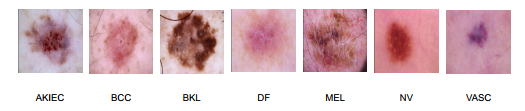
\includegraphics[width=1\linewidth]{Definitions/DataDistribution}
	\caption{Example image of each class}
	\label{fig:datadistribution}
\end{figure}
More than 50 percent of lesions are confirmed through histopathology (HISTO), the ground truth for the rest of the cases is either follow-up examination (FOLLOWUP), expert consensus (CONSENSUS), or confirmation by in-vivo confocal microscopy (CONFOCAL). On the other hand, before being used for training the whole data is shuffled then split into two part. $90$ percent and $10$ percent of the data is used for training and validating respectively.

In the previous paper\cite{03358}, the image data is augmented for all class, the number of image increase to 18015 images. Since, this data is imbalanced, using augmented data may cause the problem of well classify on the majority of class. In this paper, instead of augmenting data, metadata is used. The way of processing metadata is discuss in MetaData section. Images in this dataset has the type of $RGB$ and shape of (450, 600). However, Each backbone need the different input size of image as well as the range of pixel value. DenseNet201\cite{06993} require the input pixels values are scaled between $0$ and $1$ and each channel is normalized with respect to the ImageNet dataset. In Resnet50 and Resnet152\cite{03385}\cite{05027}, the images are converted from $RGB$ to $BGR$, then each color channel is zero-centered with respect to the ImageNet dataset, without scaling. InceptionResNetV2\cite{11946}, on the other hand, will scale input pixels between $-1$ and $1$. Similarly, three versions of MobileNet\cite{04861}\cite{04381}\cite{02244}, NasNetMobile and NasNetLarge\cite{07012} require the input pixel is in range of $-1$ and $1$. 
\subsubsection{Metadata}
The HAM10000 dataset\cite{10417} also contain the metadata of patient including gender, age, and the capturing position. During the data exploration term, the age category miss 57 data points, which is decided to remove this 57 samples. In the gender and capturing position category contain some samples of unknown. Instead of removing, these "unknowns" data points is kept and considered as "prefer not to say". Besides, the label of the whole data is preprocessed into one-hot vector.
\subsection{Model Schema}
\subsubsection{Input Schema}
Using metadata as another input is not new. In paper\cite{03910}, they decide to keep the missing value and set its value to $0$. The sex and anatomical site are categorical encoded. The age, on the other hand is numerical normalized. After processing, the metadata is fed into a two-layer neural network with 256 neurons each. Each layer contains batch normalization, a ReLU\cite{08375} activation and dropout with $p = 0.4$. The network’s output is concatenated with the CNN’s feature vector after global average pooling. Especially, they use a simply data augmentation strategy to address the problem of missing values in metadata. During training, they randomly encode each property as missing with a probability of $p = 0.1$. 

In this paper, the unknowns is kept as a type as discussed in Metadata section. Sex, anatomical site and age are also category encoded and numerical normalized, respectively. After processing, the metadata is then concatenated and fed into a dense layer of 4096 neurons. Finally, this this dense layer is then concatenate with the output of Soft-Attention which is then discussed in Soft-Attention section. The Input schema is described as follow:\\
\begin{figure}[h]
	\centering
	\includegraphics[width=0.7\linewidth]{"Definitions/Input Schema"}
	\caption{Input Schema}
	\label{fig:input-schema}
\end{figure}\\
Image data, on the other hand after being preprocessed, is fed directly into the backbone model. 
\subsubsection{Soft-Attention}
Applying the Soft-Attention layer in deep learning is not a new approach. Soft-Attention has been used in various applications: image caption generation in \cite{03044} and handwriting verification in \cite{202017} respectively. In skin lesion classification, Soft-Attention is used to increase the performance of the model as described in \cite{03358}. Soft-Attention can ignore irrelevant areas of the image by multiplying the corresponding feature maps with low weights. The function below describes the flow of the Soft-Attention module:
\[
f_{sa} = \gamma t\sum_{k=1}^{K}softmax(W_k * t)
\]

In order to apply Soft-Attention, there are two main steps. Firstly, the input tensor is put in grid-based feature extraction from the high-resolution image, where each grid cell is analyzed in the whole slide to generate a feature map\cite{08513}. This feature map called $t \in R^{h \times w \times d}$ where $h, w, \text{and } d$ is the shape of tensor generated by a Convolution Neural Network(CNN), is then input to a 3D convolution layer whose weights is $W_k \in R^{h \times w \times d \times K}$. The output of this convolution is normalized using the softmax function to generate K = 16 attention maps. These $16$ attention maps are aggregated to produce a weight function called $\alpha$. This $\alpha$ function is then multiplied with feature tensor $t$ and scaled by $\gamma$, a learnable scalar. Finally, the out of Soft-Attention function $f_{sa}$ is the concatenation of the beginning feature tensor $t$ and the scaled attention maps. 
\begin{figure}[h]
	\centering
	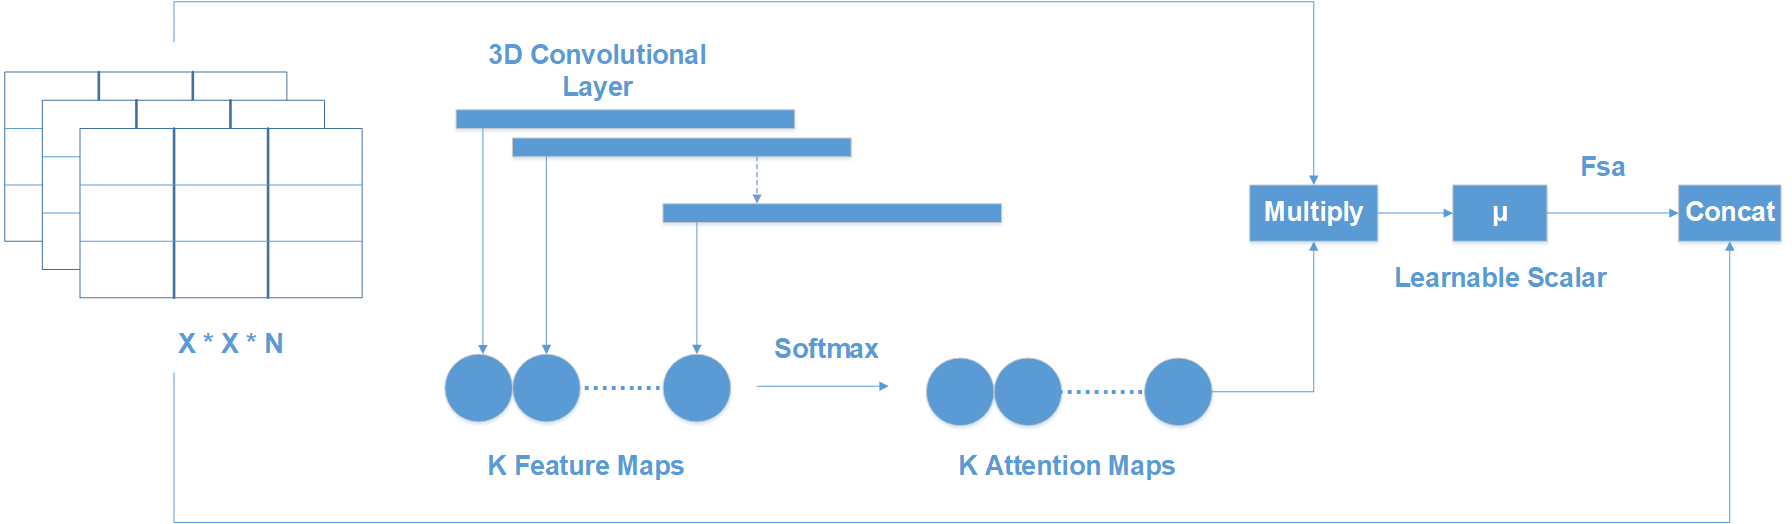
\includegraphics[width=1\linewidth]{Definitions/SoftAttention}
	\caption{Soft-Attention Module}
	\label{fig:softattention}
\end{figure}
In this paper, the Soft-Attention layer is applied in the same way in this paper\cite{03358}. The Soft-Attention module is described in the following diagram:
\FloatBarrier
\begin{figure}[h]
	\centering
	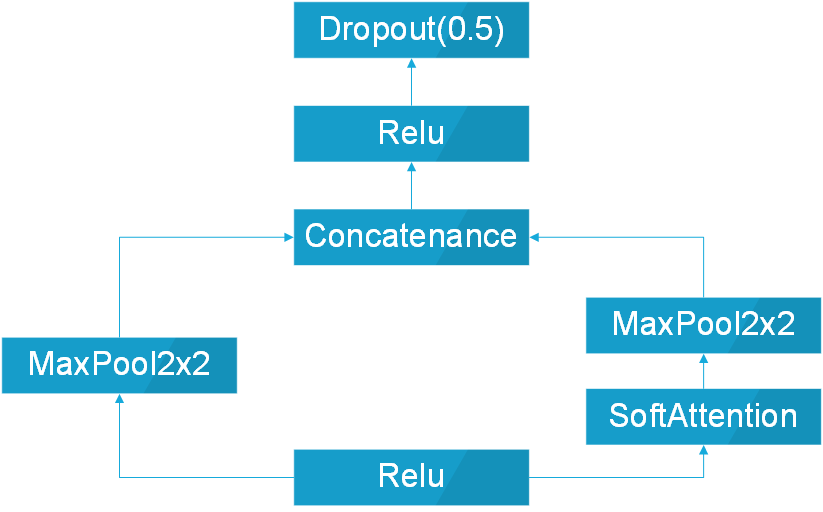
\includegraphics[width=0.5\linewidth]{Definitions/SoftAttentionBlock}
	\caption{Soft-Attention Module}
	\label{fig:softattentionblock}
\end{figure}
\FloatBarrier
\subsubsection{Backbone Model Architecture}
In this paper, the backbone models used in this paper are DenseNet201\cite{06993}, Inception\cite{00567}, MobileNets\cite{04861}\cite{04381}\cite{02244}, ResNet\cite{03385}\cite{05027}, and NasNet\cite{07012}. The combination of DenseNet201, InceptionResNetV2 and Soft-Attention layer are both tested by the previous paper\cite{03358} with a great performance. Otherwise, Resnet50 also well classify but with much less number of parameter and depth than based on its f1-score and precision stated. Therefore, in this paper, the performance of the model Resnet152 and NasnetLarge which has the larger number of parameter and depth is analyzed. On the other hand, three version of MobileNet and the NasnetMobile will also be analyzed which has a small number of parameter and depth.  
\FloatBarrier
\begin{table}[ht]
	\centering
	\begin{tabular}{|c | c c c|} 
		\hline
		Model & Size(MB) & Parameters & Depth \\ 
		\hline
		Resnet50 & 98 & 25.6M & 107 \\ 
		\hline
		Resnet152 & 232 & 60.4M & 311 \\ 
		\hline
		DenseNet201 & 80 & 20.2M & 402 \\
		\hline
		InceptionResNetV2 & 215 & 55.9M & 449 \\
		\hline
		MobileNet & 16 & 4.3M & 55 \\ 
		\hline
		MobileNetV2 & 14 & 3.5M & 105 \\ 
		\hline
		MobileNetV3Small & Unknown & 2.5M & 88 \\ 
		\hline
		MobileNetV3Large & Unknown & 5.5M & 118 \\
		\hline
		NasnetMobile & 23 & 5.3M & 308 \\
		\hline
		NasnetLarge & 343 & 88.9M & 533 \\ 
		\hline
	\end{tabular}
	\caption{Size and Parameters and Depth of backbone model used in this paper}
	\label{table:2}
\end{table}
\FloatBarrier

\subsubsection{Model}
The whole architecture of the model used for image feature extraction is applied in the same way in paper \cite{03358}. Metadata branch, otherwise is preprocessed before feeding into a dense layer then concatenate with the output of Soft-Attention layer. It is described in the figure below:
\begin{figure}[h]
	\centering
	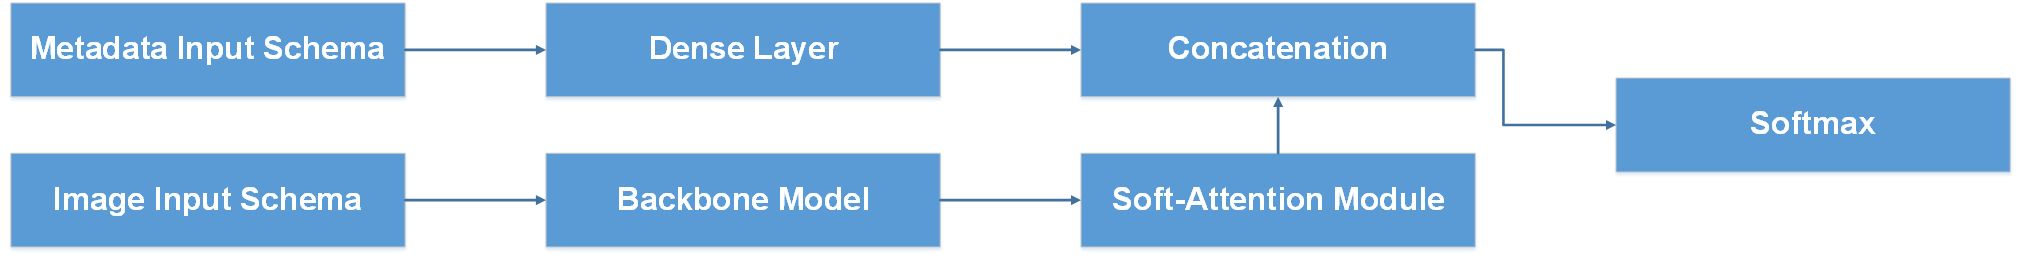
\includegraphics[width=1\linewidth]{Definitions/MainModel}
	\caption{Overall Model Architecture}
	\label{fig:mainmodel}
\end{figure}

\subsection{Loss Function}
The loss function used in this paper is categorical cross-entropy. Consider $X = [x_1, x_2, \dots, x_n]$ as the input feature, $\theta = [\theta_1, \theta_2, \dots, \theta_n]$. Let $N$, and $C$ is the number of training examples and number of class respectively. The categorical cross-entropy loss is presented as:
\[L(\theta, x_n) = -\frac{1}{N}\sum_{c=1}^{C}\sum_{n=1}^{N}W_c\times y^c_n \times \log(\hat{y}^c_n)\]
where $\hat{y}^c_i$  is the output of model and $y^c_i$ is the target that the model should return, $W_c$ is the weight of class $c$. Since the dataset face the imbalanced problem then I applied the class weight for the loss. This formula below is used to calculate the class weight:
\[W = N \odot D\]
\[D = \begin{bmatrix}
	\frac{1}{C \times  N_1} & \frac{1}{C \times  N_2} & \dots & \frac{1}{C \times  N_n}\\
\end{bmatrix} = \frac{1}{C} \odot \begin{bmatrix}
	\frac{1}{N_1} & \frac{1}{N_2} & \dots & \frac{1}{N_n}\\
\end{bmatrix}\]
where $N$ is the number of training sample, $C$ is the number of class, $N_i$ is the number of sample in each class $i$. $D$ is the matrix contain the inverse of $C \times N_i$. 
\subsection{Evaluation Metrics}
\begin{figure}[!htb]
	\begin{minipage}{0.48\textwidth}
		\centering
		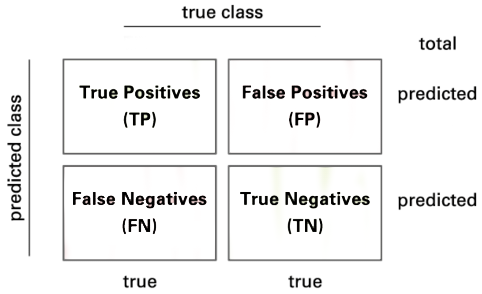
\includegraphics[width=1.1\linewidth]{Definitions/Confusion-matrix}
		\caption{Confusion Matrix}\label{Fig:Data1}
	\end{minipage}\hfill
	\begin{minipage}{0.48\textwidth}
		\centering
		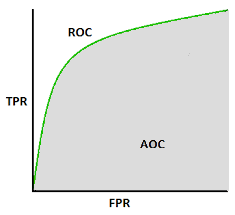
\includegraphics[width=.7\linewidth]{Definitions/AUC}
		\caption{Area Under the Curve}\label{Fig:Data2}
	\end{minipage}
\end{figure}
In this paper, the model is evaluated by using the confusion matrix and related metrics. The figure 4 illustrates the presentation of a $2 \times 2$ confusion matrix used for $2$ class. Consider a confusion matrix $A$ with $C$ number of class. Let $A^i$ and $A^j$ is the set of $A$ rows and columns respectively. 
\[
A = \begin{bmatrix}
	a_{11} & a_{12} & \dots & a_{1j} \\
	a_{21} & a_{22} & \dots & a_{2j} \\
	\vdots & \vdots	&  & \vdots\\
	a_{i1} & a_{i2} & \dots & a_{ij} 
\end{bmatrix}
\]

The True Positive(TP) of all class in this case is the main diagonal of the matrix $A$. The following method are used to calculate the False Positives(FP), False Negatives(FN), and True Negatives(TN) of all class:
\[
FP = -TP + \sum_{k=1}^{i}A^i_k \hspace{1cm} FN = -TP + \sum_{k=1}^{j}A^j_k
\]
\[
TN_c = \sum_{i=1}^{C}\sum_{j=1}^{C}a_{ij} - \left[ \sum_{k=1}^{i}A^i_{i=c k} + \sum_{k=1}^{j}A^j_{j=c k} \right] + a_{i=c j=c} \implies TN = \begin{bmatrix}
	TN_1 & TN_2 & \dots & TN_c
\end{bmatrix}
\]
Then, the model is evaluated by the following metrics:
\[\text{Sensitivity(Sens)} = \frac{TP}{TP + FN} \hspace{1cm} \text{Specificity(Spec)} = \frac{TN}{TN + FP}\]
\[\text{Precision} = \frac{TP}{TP + FP} \hspace{1cm} \text{F1 Score} = \frac{2 \times TP}{2 \times TP + FP + FN + TN}\]
\[\text{Accuracy} = \frac{TP + TN}{TP + FP + FN + TN} \hspace{1cm} \text{Balanced Accuracy} = \frac{\text{Sens} + \text{Spec}}{2}\]
The last metric is the $AUC$ score standing for Area Under the Curve which is the Receiver Operating Curve(ROC) that indicate the probability of TP versus the probability of FP.  
\subsection{Traning}
Before training, the dataset is split into three sub datasets including training, validation, and testing. In this paper, the graphic card that is used to train is Nvidia RTX TitanV.\\
All the model in this paper is trained with Adam Optimizer\cite{6980}. The initial learning rate is set to $0.001$, an learning rate reduction schedule is setup with the minimum learning rate is $0.0000001$ with the factor of $0.2$, the epsilon argument of the optimizer is set to $0.1$. On the other hand, Early Stopping is also set up, if the accuracy of validation set dose not increase after 25 epochs, the training will stop. 

%%%%%%%%%%%%%%%%%%%%%%%%%%%%%%%%%%%%%%%%%%
\section{Results}
The accuracy of all model is presented in the figure below:
\begin{table}[h]
	\centering
	\begin{tabular}{| c | c | c | c |}
		\hline
		InceptionResNetV2 & DenseNet201 & ResNet50 & VGG16 \\
		\hline
		0.93 & 0.91 & 0.92 & 0.88\\
		\hline
	\end{tabular}
	\caption{Accuracy of the model with augmented data}
	\label{table:3}
\end{table}
\begin{table}[h]
	\centering
	\begin{tabular}{| c | c | c | c | c |}
		\hline
		InceptionResNetV2 & DenseNet201 & ResNet50 & Resnet152 & MobileNetV2\\
		\hline
		0.89 & 0.89 & 0.70 & 0.57 & 0.81\\
		\hline
	\end{tabular}
\end{table}
\begin{table}[h]
	\centering
	\begin{tabular}{| c | c | c | c |}
		\hline
		MobileNetV3Large & MobileNetV3Small & NasNetLarge & NasNetMobile\\
		0.84 & 0.78 & 0.86 & 0.86\\
		\hline
	\end{tabular}
	\caption{Accuracy of the model with metadata}
	\label{table:4}
\end{table}
According to the Table 3 and 4, it is clear that the model trained with augmented data has a higher accuracy than the model trained with metadata only. While InceptionResNetV2 and DenseNet201 trained with augmented data have accuracy of $0.93$ and $0.91$ respectively, their training with metadata has both the accuracy of $0.89$. Furthermore, Resnet50 trained with augmented data has the accuracy that outperform the Resnet50 and is twice as high as Resnet152 trained with metadata. On the other hand, mobile model including MobileNetV2, MobileNetV3Large, and NasNetMobile, even though has a much smaller number of parameters and depth than the other model, they have a quite good accuracy of $0.81$, $0.84$, $0.86$, respectively. This term will be discussed later on. Since, the model trained with augmented data have high accuracy, when their f1-score and the recall score of models are analyzed, it turns out that models trained with augmented data have imbalanced f1-scores according to table 5. As a results, augmented data model dose not classify well on all class as InceptionResNetV2 trained on augmented data have $0.29$ f1-score on class df while InceptionResNetV2 trained on metadata and the new weight loss can classify well in a balanced way. 
\begin{table}[h]
	\centering
	\begin{tabular}{|c | c | c | c | c | c | c | c | c|} 
		\hline
		Model & akiec & bcc & bkl & df & mel & nv & vasc & Mean \\
		\hline
		\thead{DenseNet201 +\\ Augmented Data} & 0.67 & 0.78 & 0.64 & 0.67 & 0.61 & 0.96 & 0.91 & 0.74 \\ 
		\hline
		\thead{InceptionResNetV2 +\\ Augmented Data} & 0.69 &	0.88 & 0.77 & 0.29 & 0.66 & 0.98 & 1 & 0.75\\
		\hline
		\thead{Resnet50 +\\ Augmented Data} & 0.53 & 0.86 & 0.68 & 0.67 & 0.57 & 0.97 & 0.95 & 0.74\\
		\hline 	
		\thead{VGG16 +\\ Augmented Data} & 0.65 & 0.7 & 0.52 & 0.4 & 0.53 & 0.95 & 0.95 & 0.67\\ 
		\hline		
		\thead{DenseNet201 +\\Metadata and WeightLoss} & \textbf{0.84} & 0.77 & \textbf{0.81} & \textbf{0.83} & \textbf{0.69} & 0.94 & 0.97 & \textbf{0.83}\\
		\hline
		\thead{InceptionResNetV2 +\\Metadata and WeightLoss} & 0.77 & 0.83 & \textbf{0.83} & 0.64 & \textbf{0.75} & 0.94 & 0.7 & \textbf{0.81}\\
		\hline
		\thead{Resnet50 +\\Metadata and WeightLoss} & 0.49 & 0.59 & 0.55 & 0.36 & 0.45 & 0.83 & 0.8 & 0.58\\
		\hline
		\thead{Resnet152 +\\Metadata and WeightLoss} & 0.42 & 0.38 & 0.41 & 0.15 & 0.4 & 0.75 & 0.75 & 0.46\\
		\hline
		\thead{NasNetLarge +\\Metadata and WeightLoss} & 0.79 & 0.79 & 0.8 & 0.74 & 0.65 & 0.92 & 0.92 & \textbf{0.80}\\
		\hline
		\thead{MobileNetV2 +\\Metadata and WeightLoss} & 0.68 & 0.79 & 0.66 & 0.78 & 0.54 & 0.9 & \textbf{0.9} & 0.75\\
		\hline
		\thead{MobileNetV3Large +\\Metadata and WeightLoss} & 0.72 & 0.76 & 0.75 & 0.92 & 0.58 & 0.92 & \textbf{0.92} & 0.79\\
		\hline
		\thead{MobileNetV3Small +\\Metadata and WeightLoss} & 0.6 & 0.72 & 0.61 & 0.75 & 0.47 & 0.89 & \textbf{0.89} & 0.70\\
		\hline
		\thead{NasNetMobile +\\Metadata and WeightLoss} & 0.76 & 0.74 & 0.78 & 0.73 & 0.63 & 0.93 & \textbf{0.93} & 0.78\\
		\hline
	\end{tabular}
	\caption{F1-Score of each class and the mean f1-score of each model}
	\label{table:5}
\end{table}

However, only DenseNet201, InceptionResNetV2, and NasNetLarge whose depth are equal or larger than 400 have balanced f1-score on class. The others still face the imbalanced term. Since this dataset is not balanced, therefore using augmented data can make the model more  bias to the class which has larger sample. Using the metadata, though still make the model bias, it dose contributes to the improvement of  the performance of the model.

\begin{table}[h]
	\centering
	\begin{tabular}{|l | c | c | c | c | c | c | c | c|} 
		\hline
		Model & akiec & bcc & bkl & df & mel & nv & vasc & Mean \\
		\hline
		\thead{DenseNet201 +\\ Augmented Data} & 0.52 & 0.77 & 0.58 & 0.5 & 0.71 & 0.97 & 1 & 0.72\\ 
		\hline
		\thead{InceptionResNetV2 +\\ Augmented Data} & 0.52 & 0.88 & 0.83 & 0.17 & 0.65 & 0.98 & 1 & 0.71\\
		\hline
		\thead{Resnet50 +\\ Augmented Data} & 0.43 & 0.85 & 0.7 & 0.5 & 0.47 & 0.98 & 0.9 & 0.69\\
		\hline 	
		\thead{VGG16 +\\ Augmented Data} & 0.61 & 0.81 & 0.44 & 0.44 & 0.68 & 0.95 & 0.9 & 0.69\\ 
		\hline		
		\thead{DenseNet201 +\\Metadata and WeightLoss} & \textbf{0.85} & 0.75 & 0.78 & 0.83 & 0.63 & 0.96 & \textbf{1} & \textbf{0.82}\\
		\hline
		\thead{InceptionResNetV2 +\\Metadata and WeightLoss} & \textbf{0.82} & 0.84 & 0.81 & 0.67 & 0.7 & 0.95 & 0.93 & \textbf{0.81}\\
		\hline
		\thead{Resnet50 +\\Metadata and WeightLoss} & 0.67 & 0.63 & 0.54 & 0.83 & 0.63 & 0.74 & 0.86 & 0.70\\
		\hline
		\thead{Resnet152 +\\Metadata and WeightLoss} & 0.51 & 0.49 & 0.35 & 0.76 & 0.47 & 0.63 & 0.48 & 0.52\\
		\hline
		\thead{NasNetLarge +\\Metadata and WeightLoss} & 0.73 & 0.71 & \textbf{0.83} & \textbf{0.92} & 0.59 & 0.9 & 0.93 & \textbf{0.81}\\
		\hline
		\thead{MobileNetV2 +\\Metadata and WeightLoss} & 0.7 & 0.86 & 0.72 & 0.75 & 0.58 & 0.86 & \textbf{1} & 0.78\\
		\hline
		\thead{MobileNetV3Large +\\Metadata and WeightLoss} & 0.72 & 0.76 & 0.75 & \textbf{0.92} & 0.58 & 0.92 & 0.92 & \textbf{0.80}\\
		\hline
		\thead{MobileNetV3Small +\\Metadata and WeightLoss} & 0.76 & 0.84 & 0.68 & \textbf{1} & 0.52 & 0.82 & 0.93 & 0.79\\
		\hline
		\thead{NasNetMobile +\\Metadata and WeightLoss} & \textbf{0.82} & 0.73 & \textbf{0.83} & \textbf{0.92} & 0.53 & 0.93 & 0.93 & \textbf{0.81}\\
		\hline
	\end{tabular}
	\caption{Recall score of each class and the mean recall score of each model}
	\label{table:6}
\end{table}

This problem is also true with the recall score according to table 6. DenseNet201, InceptionResNetV2, ResNet50, VGG16 trained with augmented data has expected value of recall of $0.72$, $0.71$, $0.69$, $0.69$, respectively, while the combination of InceptionResNetV2, Metadata and the new weight loss function achieve the expected value of recall: $0.82$.

As the results, metadata does improve the model performance by reducing the amount of data needed for achieving nearly the expected results. On the other hand, the reason why the model become much more balanced is the weighted loss function. Weight loss function has ability to solve the imbalanced class samples by adding a weight related to the number of samples in each class. Therefore, DenseNet201, InceptionResNetV2 trained with the new weighted loss function have recall in akiec of $0.85$. $0.82$, respectively, as opposed to their training in akiec without weighted loss function. MobileV3large, MobileV3Small, NasNetLarge and NasNetMobile whose standard deviation is less than $0.15$ outperform others on classifying class df with the recall score of $0.92$, $1$, $0.92$, $0.92$, separately.

Another interesting point found during the experiment is that MobileNetV2, MobileNetV3 and NasNetMobile have small number of parameters and depth, though have relative good performance. The table 8 illustrates the deeper analyzing of the three models. It's clear that MobileNetV3Large and NasNetMobile are the two best performance model.
\FloatBarrier
\begin{table}[ht]
	\centering	
	\begin{tabular}{|l | c | c | c | c|} 
		\hline
		Model & \cite{04381} & \cite{02244}Small & \cite{02244}Large & \cite{07012}Mobile\\
		\hline
		Accuracy(avg) & 0.81 & 0.78 & 0.84 & \textbf{0.86}\\
		\hline
		Balanced Accuracy(avg) & 0.86 & 0.87 & 0.87 & \textbf{0.88}\\ 
		\hline
		Precision(avg) & 0.71 & 0.63 & \textbf{0.75} & 0.73\\
		\hline
		F1-score(avg) & 0.75 & 0.70 & \textbf{0.79} & 0.78\\
		\hline
		Sensitivity(avg) & 0.78 & 0.79 & 0.80 & \textbf{0.81}\\ 
		\hline
		Specificity(avg) & 0.95 & 0.95 & 0.95 & \textbf{0.96}\\
		\hline
		ROC-AUC-score(avg) & 0.96 & 0.95 & 0.96 & \textbf{0.97}\\
		\hline
	\end{tabular}
	\caption{Deeper analyzing of mobile model}
	\label{table:7}
\end{table}
\FloatBarrier
Nevertheless, MobileNetV3Large has less number of parameters and depth than NasNetMobile according to the table 2. Therefore, at the end of this experiment, I decide to configure the MobileNetV3Large to construct an optimized model. The result of this experiment is illustrated in table 9.
\FloatBarrier
\begin{table}[ht]
	\centering
	\begin{tabular}{|l | c |}
		\hline
		Model & Accuracy\\
		\hline
		MobileNetV3Large-Layer[:270] + Soft-Attention + Metadata & 0.71 \\
		\hline
		MobileNetV3Large-Layer[:266] + Soft-Attention + Metadata  & 0.73 \\
		\hline
		MobileNetV3Large-Layer[:260] + Soft-Attention + Metadata  & 0.77 \\
		\hline
		MobileNetV3Large-Layer[:251] + Soft-Attention + Metadata  & 0.79 \\
		\hline
		MobileNetV3Large-Layer[:246] + Soft-Attention + Metadata  & 0.84 \\
		\hline
		MobileNetV3Large-Layer[:246] + Soft-Attention + Dense(512) + Metadata & 0.85 \\
		\hline
		MobileNetV3Large-Layer[:240] + Soft-Attention + Metadata  & \textbf{0.86}\\
		\hline
		MobileNetV3Large-Layer[:230] + Soft-Attention + Metadata  & 0.84 \\
		\hline
		MobileNetV3Large-Layer[:230] + Soft-Attention & 0.85 \\ 
		\hline
		MobileNetV3Large & 0.85 \\ 
		\hline
	\end{tabular}
	\caption{Deeper analyzing of MobileNetV3Large Model}
	\label{table:8}
\end{table}
\FloatBarrier
The Table 9 demonstrate that the Soft-Attention and the metadata have a good effect on the model. Otherwise, Adding a dense layer does not increase the model performance. The best MobileNetV3Large model architecture is the combination of MobileNetV3Large replaced from $241^{th}$ layer to the rest by Soft-Attention layer and the metadata, which peak the model performance of $0.86$ accuracy rate. 
\FloatBarrier
\begin{table}[ht]
	\centering
	\begin{tabular}{| l | c |}
		\hline
		Accuracy & 0.86\\
		\hline
		Precision(avg) & 0.86\\
		\hline
		F1-score(avg) & 0.86\\
		\hline
		Sensitivity(avg) & 0.86\\
		\hline
		Specificity(avg) & 0.95\\
		\hline
		ROC AUC Score(avg) & 0.98\\
		\hline
	\end{tabular}
	\caption{Performance of MobileNetV3Large}
	\label{table:9}
\end{table}
\FloatBarrier
\begin{table}[ht]
	\centering
	\begin{tabular}{| l | c | c | c |}
		\hline
		Model & MobileNetV3Large & DenseNet201 & InceptionResnetV2\\
		\hline
		No. Parameters & \textbf{5.5M} & 20.2M & 55.9M\\
		\hline
		Depth & \textbf{118} & 402 & 449\\
		\hline
		Accuracy & 0.86 & 0.89 & 0.90\\
		\hline
		Time Prediction(s/epochs) & \textbf{116} & 1000 & 3500 \\
		\hline
	\end{tabular}
	\caption{How Performance of MobileNetV3Large be optimized}
	\label{table:11}
\end{table}
\FloatBarrier
\section{Conclusions}
In this paper, my objective is to analyze the effect of metadata on the performance of model as well as identifying whether metadata can make the model less imbalanced or not. On the other hand, I also try to construct an optimized and balanced model that can be used on mobile phone or electronic devices. The experiment shown that metadata improve the model performance, the factor that make the model much more imbalanced is the augmented data. This problem can be solve quite absolutely by using aforementioned weighted loss function. Using weighted loss function make the expected value of model f1-score increase. At the end of the experiment, mobile model is found that can achieve great performance without either the large number of parameters or depth.  

\vspace{6pt} 

%%%%%%%%%%%%%%%%%%%%%%%%%%%%%%%%%%%%%%%%%%
%% optional
%\supplementary{The following supporting information can be downloaded at:  \linksupplementary{s1}, Figure S1: title; Table S1: title; Video S1: title.}

% Only for the journal Methods and Protocols:
% If you wish to submit a video article, please do so with any other supplementary material.
% \supplementary{The following supporting information can be downloaded at: \linksupplementary{s1}, Figure S1: title; Table S1: title; Video S1: title. A supporting video article is available at doi: link.}

%%%%%%%%%%%%%%%%%%%%%%%%%%%%%%%%%%%%%%%%%%
\authorcontributions{In this paper, I am the only author, therefore I need to do all things including research, implementation, analyze data, writing draft resolution}

\funding{This research received no external funding}

\institutionalreview{Not applicable}

\informedconsent{Not applicable}

\dataavailability{In this section, please provide details regarding where data supporting reported results can be found, including links to publicly archived datasets analyzed or generated during the study. Please refer to suggested Data Availability Statements in section ``MDPI Research Data Policies'' at \url{https://www.mdpi.com/ethics}. If the study did not report any data, you might add ``Not applicable'' here.} 

\acknowledgments{I would like to express my special thanks of gratitude to my teacher, Dr.Nguyen Viet Dung (dung.nguyenviet1@hust.edu.vn) who gave me the golden support to do this wonderful project. He gave a chance to use High GPU computing computer for AI Training. Otherwise, he also gave me recommendation on how to implement experiment to make a good conclusion such as what I should focus on, what I need to investigate, which metrics I should consider.}

\conflictsofinterest{The authors declare no conflict of interest.} 

%%%%%%%%%%%%%%%%%%%%%%%%%%%%%%%%%%%%%%%%%%
%% Optional
\sampleavailability{Samples of the compounds ... are available from the authors.}

%% Only for journal Encyclopedia
%\entrylink{The Link to this entry published on the encyclopedia platform.}

\abbreviations{Abbreviations}{
The following abbreviations are used in this manuscript:\\

\noindent 
\begin{tabular}{@{}ll}
CAD & Computer aided diagnosis\\
AI & Artificial Intelligence\\
AKIEC & Actinic keratoses and intraepithelial carcinoma or Bowen's disease\\
BCC & Basal Cell Carcinoma\\
BKL & Benign Keratosis-like Lesions\\
DF & Dermatofibroma\\
MEL & Melanoma\\
NV & Melanocytic Nevi\\
VASC & Vascular Lesions\\
HISTO & Histopathology\\
FOLLOWUP & Follow-up examination\\
CONSENSUS & Expert Consensus\\
CONFOCAL & Confocal Microscopy\\
RGB & Red Green Blue\\
BGR & Blue Green Red\\
TP & True Positives\\
FN & False Negatives\\
TN & True Negatives\\
FP & False Positives\\
Sens & Sensitivity\\
Spec & Specificity\\
AUC & Area Under the Curve\\
ROC & Receiver Operating Curve\\
\end{tabular}
}

%%%%%%%%%%%%%%%%%%%%%%%%%%%%%%%%%%%%%%%%%%
%% Optional
\begin{comment}
	\appendixtitles{no} % Leave argument "no" if all appendix headings stay EMPTY (then no dot is printed after "Appendix A"). If the appendix sections contain a heading then change the argument to "yes".
	\appendixstart
	\appendix
	\section[\appendixname~\thesection]{}
	\subsection[\appendixname~\thesubsection]{}
	The appendix is an optional section that can contain details and data supplemental to the main text---for example, explanations of experimental details that would disrupt the flow of the main text but nonetheless remain crucial to understanding and reproducing the research shown; figures of replicates for experiments of which representative data are shown in the main text can be added here if brief, or as Supplementary Data. Mathematical proofs of results not central to the paper can be added as an appendix.
	
	\begin{table}[H] 
	\caption{This is a table caption.\label{tab5}}
	\newcolumntype{C}{>{\centering\arraybackslash}X}
	\begin{tabularx}{\textwidth}{CCC}
	\toprule
	\textbf{Title 1}	& \textbf{Title 2}	& \textbf{Title 3}\\
	\midrule
	Entry 1		& Data			& Data\\
	Entry 2		& Data			& Data\\
	\bottomrule
	%\end{tabularx}
	%\end{table}
	
	\section[\appendixname~\thesection]{}
	All appendix sections must be cited in the main text. In the appendices, Figures, Tables, etc. should be labeled, starting with ``A''---e.g., Figure A1, Figure A2, etc.
\end{comment}


%%%%%%%%%%%%%%%%%%%%%%%%%%%%%%%%%%%%%%%%%%
\begin{adjustwidth}{-\extralength}{0cm}
%\printendnotes[custom] % Un-comment to print a list of endnotes

\reftitle{References}

% Please provide either the correct journal abbreviation (e.g. according to the “List of Title Word Abbreviations” http://www.issn.org/services/online-services/access-to-the-ltwa/) or the full name of the journal.
% Citations and References in Supplementary files are permitted provided that they also appear in the reference list here. 

%=====================================
% References, variant A: external bibliography
%=====================================
%\bibliography{your_external_BibTeX_file}

%=====================================
% References, variant B: internal bibliography
%=====================================
\begin{thebibliography}{999}

\bibitem[Author1(year)]{08332}
Katherine M. Li and Evelyn C. Li. Skin Lesion Analysis Towards Melanoma Detection via End-to-end Deep Learning of Convolutional Neural Networks. 
{\em Journal Abbreviation} 
{\bf 2018}.

\bibitem[Author2(year)]{03225}
Xiaohan Xing and Yuenan Hou and  Hang Li and Yixuan Yuan and Hongsheng Li and Max Q.-H. Meng Categorical Relation-Preserving Contrastive Knowledge Distillation for Medical Image Classification. 
{\em Journal Abbreviation} 
{\bf 2021}.

\bibitem[Author2(year)]{03798}
Rishu Garg and Saumil Maheshwari and Anupam Shukla Decision Support System for Detection and Classification of Skin Cancer using CNN. {\em Journal Abbreviation} {\bf 2019}.

\bibitem[Author2(year)]{09365}
Xuan Li and Yuchen Lu and Christian Desrosiers and Xue Liu Out-of-Distribution Detection for Skin Lesion Images with Deep Isolation Forest. 
{\em Journal Abbreviation} 
{\bf 2020}.

\bibitem[Author2(year)]{10348}
Amirreza Rezvantalab and Habib Safigholi and Somayeh Karimijeshni Dermatologist Level Dermoscopy Skin Cancer Classification Using Different Deep Learning Convolutional Neural Networks Algorithms. 
{\em Journal Abbreviation} 
{\bf 2021}.

\bibitem[Author2(year)]{06612}
Kyle Young and Gareth Booth and Becks Simpson and Reuben Dutton and Sally Shrapnel Dermatologist Level Dermoscopy Deep neural network or dermatologist?. {\em Journal Abbreviation} 
{\bf 2021}.

\bibitem[Author2(year)]{10417}
Philipp Tschandl and Cliff Rosendahl and Harald Kittler The HAM10000 dataset, a large collection of multi-source dermatoscopic images of common pigmented skin lesions. 
{\em Journal Abbreviation} 
{\bf 2018}.

\bibitem[Author2(year)]{05045}
Michele Alberti and Angela Botros and Narayan Schuez and Rolf Ingold and Marcus Liwicki and Mathias Seuret Trainable Spectrally Initializable Matrix Transformations in Convolutional Neural Networks. 
{\em Journal Abbreviation} 
{\bf 2019}.

\bibitem[Author2(year)]{09418}
Hemanth Nadipineni Method to Classify Skin Lesions using Dermoscopic images. {\em Journal Abbreviation} 
{\bf 2020}.

\bibitem[Author2(year)]{03910}
Nils Gessert and Maximilian Nielsen and Mohsin Shaikh and René Werner and Alexander Schlaefer Skin Lesion Classification Using Ensembles of Multi-Resolution EfficientNets with Meta Data. 
{\em Journal Abbreviation} 
{\bf 2020}.

\bibitem[Author2(year)]{11797}
Pranav Poduval and Hrushikesh Loya and Amit Sethi Functional Space Variational Inference for Uncertainty Estimation in Computer Aided Diagnosis. 
{\em Journal Abbreviation} 
{\bf 2020}.

\bibitem[Author2(year)]{01284}
Peng Yao and Shuwei Shen, Mengjuan Xu and Peng Liu and Fan Zhang and Jinyu Xing and Pengfei Shao and Benjamin Kaffenberger and Ronald X. Xu Single Model Deep Learning on Imbalanced Small Datasets for Skin Lesion Classification. 
{\em Journal Abbreviation} 
{\bf 2022}.

\bibitem[Author2(year)]{11872}
Manu Goyal and Thomas Knackstedt and Shaofeng Yan and Saeed Hassanpour Artificial Intelligence-Based Image Classification for Diagnosis of Skin Cancer: Challenges and Opportunities. 
{\em Journal Abbreviation} 
{\bf 2020}.

\bibitem[Author2(year)]{03358}
Soumyya Kanti Datta and  Mohammad Abuzar Shaikh and Sargur N. Srihari and Mingchen Gao Soft-Attention Improves Skin Cancer Classification Performance. {\em Journal Abbreviation} 
{\bf 2021}.

\bibitem[Author2(year)]{12602}
Amirreza Mahbod and Philipp Tschandl and Georg Langs and Rupert Ecker and Isabella Ellinger The Effects of Skin Lesion Segmentation on the	Performance of Dermatoscopic Image Classification
{\em Journal Abbreviation} 
{\bf 2020}.

\bibitem[Author2(year)]{03426}
Yeong Chan Lee and Sang-Hyuk Jung and Hong-Hee Won WonDerM: Skin Lesion Classification with Fine-tuned Neural Networks
{\em Journal Abbreviation} 
{\bf 2019}.

\bibitem[Author2(year)]{04803}
Zihang Dai and Hanxiao Liu and Quoc V. Le and Mingxing Tan: CoAtNet Marrying Convolution and Attention for All Data Sizes
{\em Journal Abbreviation} 
{\bf 2021}.

\bibitem[Author2(year)]{06993}
Gao Huang and Zhuang Liu and Laurens van der Maaten and Kilian Q. Weinberger: Densely Connected Convolutional Network
{\em Journal Abbreviation} 
{\bf 2018}.

\bibitem[Author2(year)]{11946}
Mingxing Tan and Quoc V. Le EfficientNet: Rethinking Model Scaling for Convolutional Neural Networks
{\em Journal Abbreviation} 
{\bf 2020}.

\bibitem[Author2(year)]{00567}
Christian Szegedy and Vincent Vanhoucke and Sergey Ioffe and Jonathon Shlens and Zbigniew Wojna Rethinking the Inception Architecture for Computer Vision
{\em Journal Abbreviation} 
{\bf 2015}.

\bibitem[Author2(year)]{04861}
Andrew G. Howard and Menglong Zhu and Bo Chen and Dmitry Kalenichenko and Weijun Wang and Tobias Weyand and Marco Andreetto and Hartwig Adam MobileNets: Efficient Convolutional Neural Networks for Mobile Vision Applications
{\em Journal Abbreviation} 
{\bf 2017}.

\bibitem[Author2(year)]{04381}
Mark Sandler and Andrew Howard and Menglong Zhu and Andrey Zhmoginov and Liang-Chieh Chen MobileNetV2: Inverted Residuals and Linear Bottlenecks
{\em Journal Abbreviation} 
{\bf 2018}.

\bibitem[Author2(year)]{02244}
Andrew Howard and Mark Sandler and Grace Chu and Liang-Chieh Chen and Bo Chen and Mingxing Tan and Weijun Wang and Yukun Zhu and Ruoming Pang and Vijay Vasudevan and Quoc V. Le and Hartwig Adam Searching for MobileNetV3
{\em Journal Abbreviation} 
{\bf 2019}.

\bibitem[Author2(year)]{03385}
Kaiming He and Xiangyu Zhang and Shaoqing Ren and Jian Sun Deep Residual Learning for Image Recognition
{\em Journal Abbreviation} 
{\bf 2015}.

\bibitem[Author2(year)]{05027}
Kaiming He and Xiangyu Zhang and Shaoqing Ren and Jian Sun Identity Mappings in Deep Residual Networks
{\em Journal Abbreviation} 
{\bf 2016}.

\bibitem[Author2(year)]{1556}
Karen Simonyan and Andrew Zisserman Very Deep Convolutional Networks for Large-Scale Image Recognition
{\em Journal Abbreviation} 
{\bf 2016}.

\bibitem[Author2(year)]{02357}
François Chollet Xception: Deep Learning with Depthwise Separable Convolutions
{\em Journal Abbreviation} 
{\bf 2017}.

\bibitem[Author2(year)]{6980}
Diederik P. Kingma, Jimmy Ba Adam: A Method for Stochastic Optimization
{\em Journal Abbreviation} 
{\bf 2017}.

\bibitem[Author2(year)]{03044}
Kelvin Xu and Jimmy Ba and Ryan Kiros and Kyunghyun Cho and Aaron Courville and Ruslan Salakhutdinov and Richard Zemel and Yoshua Bengio Show, Attend and Tell: Neural Image Caption Generation with Visual Attention 2020 17th International Conference on Frontiers in Handwriting Recognition
{\em Journal Abbreviation} 
{\bf 2016}.

\bibitem[Author2(year)]{08513}
Naofumi Tomita and Behnaz Abdollahi and Jason Wei and Bing Ren and Arief Suriawinata and Saeed Hassanpour. Attention-Based Deep Neural Networks for Detection of Cancerous and Precancerous Esophagus Tissue on Histopathological Slides
{\em Journal Abbreviation} 
{\bf 2020}.

\bibitem[Author2(year)]{02357}
Mohammad Abuzar Shaikh and Tiehang Duan and Mihir Chauhan and Sargur N. Srihari. 2020 17th International Conference on Frontiers in Handwriting Recognition
{\em Journal Abbreviation} 
{\bf 2019}.

\bibitem[Author2(year)]{8943952}
Srihari. YAOSHIANG HO AND SAMUEL WOOKEY The Real-World-Weight Cross-Entropy Loss Function: Modeling the Costs of Mislabeling 
{\em Journal Abbreviation} 
{\bf 2020}.

\bibitem[Author2(year)]{07012}
Barret Zoph, Vijay Vasudevan, Jonathon Shlens, Quoc V. Le Learning Transferable Architectures for Scalable Image Recognition 
{\em Journal Abbreviation} 
{\bf 2017}.

\bibitem[Author2(year)]{08375}
Abien Fred Agarap Deep Learning using Rectified Linear Units (ReLU) 
{\em Journal Abbreviation} 
{\bf 2019}.

\bibitem[Author2(year)]{01507}
Jie Hu, Li Shen, Samuel Albanie, Gang Sun, Enhua Wu Squeeze-and-Excitation Networks 
{\em Journal Abbreviation} 
{\bf 2019}.

\bibitem[Author2(year)]{04552v2}
Improved Regularization of Convolutional Neural Networks with Cutout Improved Regularization of Convolutional Neural Networks with Cutout 
{\em Journal Abbreviation} 
{\bf 2017}.

\end{thebibliography}

% If authors have biography, please use the format below
%\section*{Short Biography of Authors}
%\bio
%{\raisebox{-0.35cm}{\includegraphics[width=3.5cm,height=5.3cm,clip,keepaspectratio]{Definitions/author1.pdf}}}
%{\textbf{Firstname Lastname} Biography of first author}
%
%\bio
%{\raisebox{-0.35cm}{\includegraphics[width=3.5cm,height=5.3cm,clip,keepaspectratio]{Definitions/author2.jpg}}}
%{\textbf{Firstname Lastname} Biography of second author}

% For the MDPI journals use author-date citation, please follow the formatting guidelines on http://www.mdpi.com/authors/references
% To cite two works by the same author: \citeauthor{ref-journal-1a} (\citeyear{ref-journal-1a}, \citeyear{ref-journal-1b}). This produces: Whittaker (1967, 1975)
% To cite two works by the same author with specific pages: \citeauthor{ref-journal-3a} (\citeyear{ref-journal-3a}, p. 328; \citeyear{ref-journal-3b}, p.475). This produces: Wong (1999, p. 328; 2000, p. 475)

%%%%%%%%%%%%%%%%%%%%%%%%%%%%%%%%%%%%%%%%%%
%% for journal Sci
%\reviewreports{\\
%Reviewer 1 comments and authors’ response\\
%Reviewer 2 comments and authors’ response\\
%Reviewer 3 comments and authors’ response
%}
%%%%%%%%%%%%%%%%%%%%%%%%%%%%%%%%%%%%%%%%%%
\end{adjustwidth}
\end{document}

